\section{Distribution of skin-tones}
\label{sec:skin-tone-distribution}

\textbf{RQ3:} \textit{How fair the distribution of skin tone in the bollywood movies?}

To assess the prevalence and variation of skin tones across different types of roles in the Hindi film industry, we examined the distribution of luminance (L*) values extracted from the CIELAB color space. Luminance serves as a continuous proxy for skin tone lightness, with higher values indicating lighter skin.

\subsection{Luminance Distribution by Role}
This visualization shows the overall distribution of luminance values categorized by role: actors, actresses, side actors, and side actresses from 2015 to 2024. A clear separation in the density of L* values suggests that lead roles, particularly actresses, tend to cluster at higher luminance levels, indicating a preference for lighter skin tones in prominent casting decisions.

\begin{figure}[!htb]
    \centering
    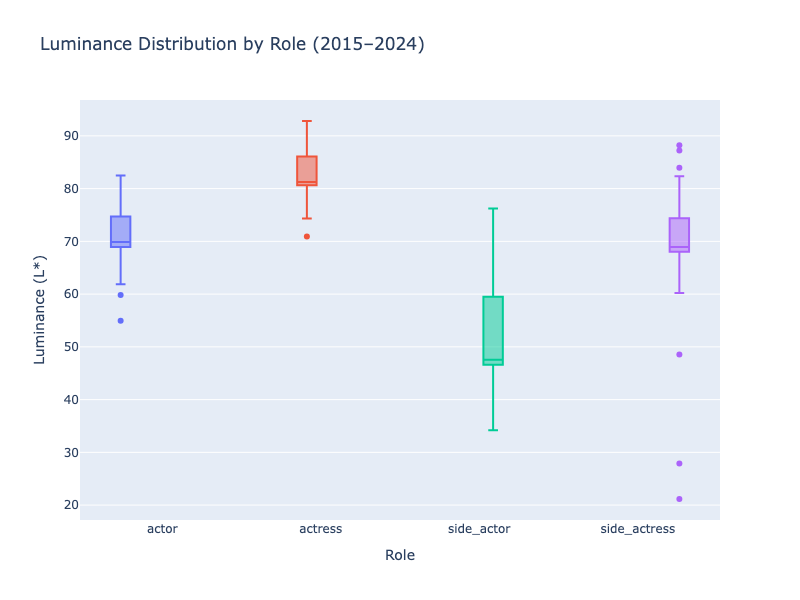
\includegraphics[width=0.7\textwidth]{luminance_distribution_by_role.png}
    \caption{\textit{Luminance distribution of actors and actresses in Bollywood movies from 2015 to 2024.}}
    \label{fig: Luminance Distribution by Role}
\end{figure}

\subsection{Luminance Histogram by Role}
Histograms provide further insight into the frequency distribution of luminance values within each role category. The data shows that side actors and side actresses display a broader spread of luminance values, while lead roles have more tightly clustered distributions with peaks at higher luminance levels. This points toward a more restrictive appearance norm for leads.
\begin{figure}[!htpb]
    \centering
    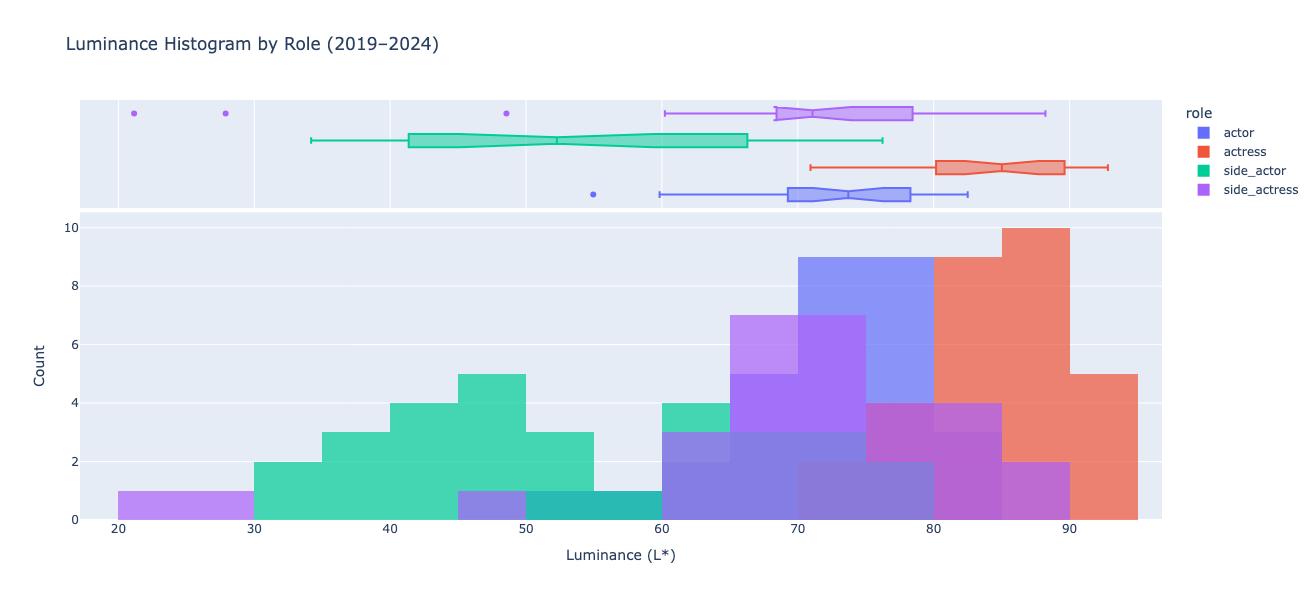
\includegraphics[width=0.8\textwidth]{luminance_histogram_by_role.png}
    \caption{\textit{Luminance histogram of actors and actresses in Bollywood movies from 2019 to 2024.}}
    \label{fig: Luminance Histogram by Role}
\end{figure}

\subsection{Luminance Distribution with Percentile Overlays}
To visualize the statistical spread within each role, we plotted the luminance values with percentile overlays (e.g., 10th, 25th, 50th, 75th, and 90th percentiles). This plot reveals not only central tendencies but also the range of variation. Lead roles show a narrower interquartile range and higher median luminance compared to side roles, reinforcing the observation that lighter skin is more typical among central characters.
\begin{figure}[!htpb]
    \centering
    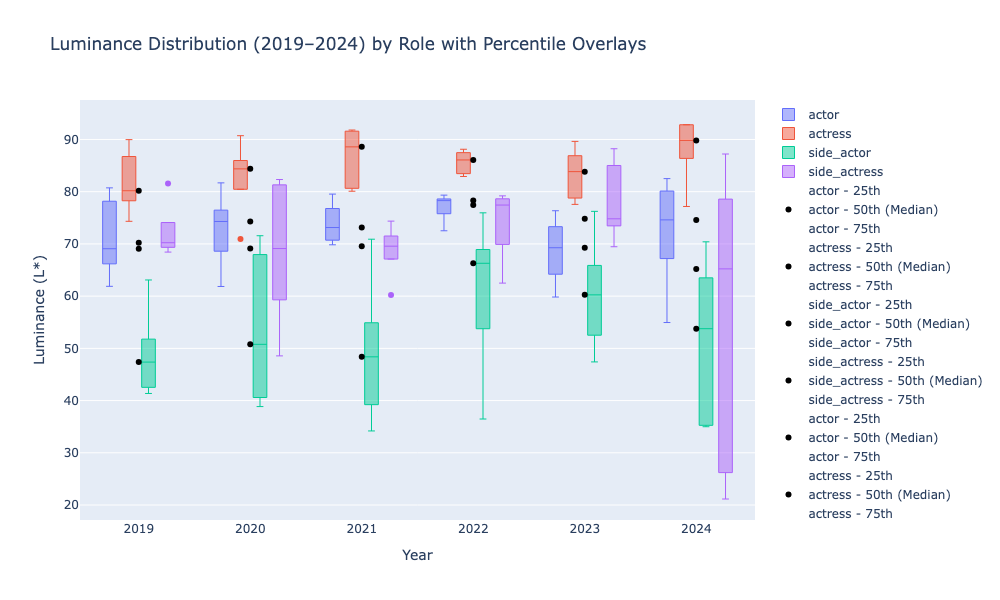
\includegraphics[width=0.8\textwidth]{luminance_distribution_by_role_with_percentile_overlays.png}
    \caption{\textit{Luminance distributions by role in Bollywood movies with percentile overlays from 2019 to 2024.}}
    \label{fig: Luminance percentile overlays by Role}
\end{figure}

\subsection{Average Luminance Over Time by Role}
We also tracked the average luminance of each role across the years 2019 to 2024 to observe any temporal trends. The results suggest that the average luminance of lead roles has remained relatively high and stable, indicating a persistent aesthetic bias over time. Side roles exhibit more fluctuation and lower mean values, further emphasizing the role-based disparity in skin tone representation.
\begin{figure}[!htpb]
    \centering
    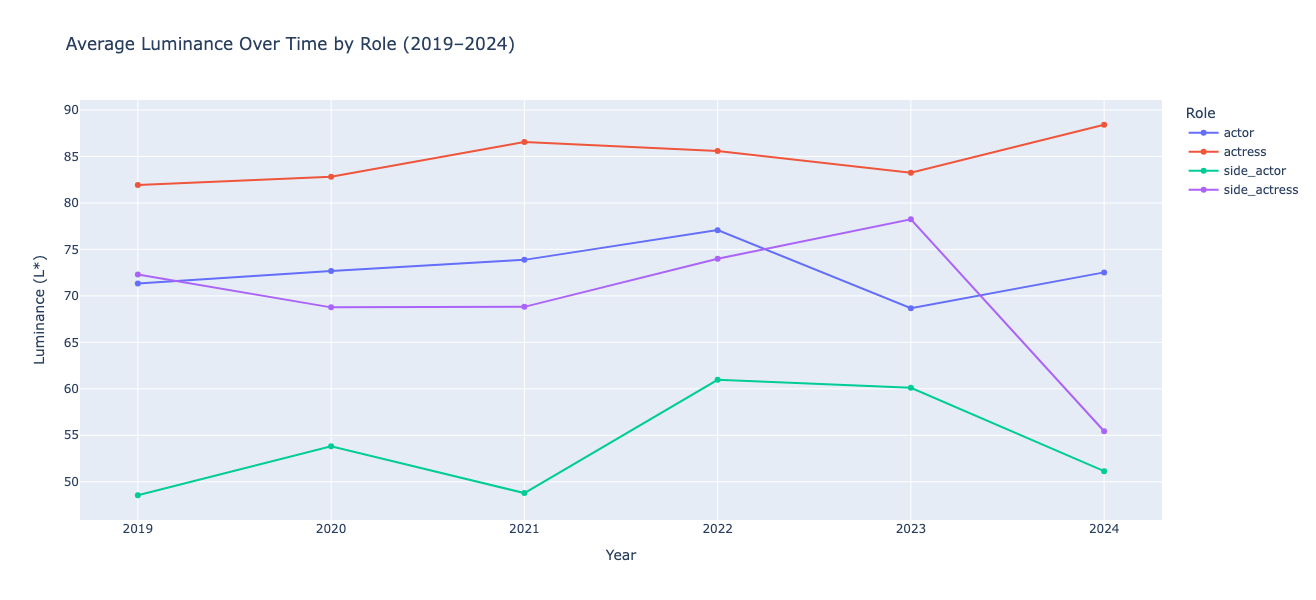
\includegraphics[width=0.8\textwidth]{average_luminance_over_time_by_role.png}
    \caption{\textit{Average luminance over time by roles from 2019 to 2024.}}
    \label{fig: Luminance average by Role}
\end{figure}
